\documentclass{article}
\usepackage{graphicx} % Required for inserting images
\usepackage{ragged2e}
\usepackage{placeins}
\usepackage{longtable}
\usepackage{booktabs}
\usepackage{caption}
\usepackage{array}
\usepackage{enumitem}

\title{Project Documentation 1}
\author{
    Akash Srinivasan \and
    Caden Roberts \and
    Jhovanny Uribe \and
    Andy Vo \and
    Ethan Cesario \and
    Aliyaa Islam
}
\date{\textbf{January 2025}}
\begin{document}
\RaggedRight

\maketitle

\section{Client}

\begin{itemize}
    \item Health Insurance Companies
\end{itemize}

\section{Need Statement}
\begin{itemize}
    \item People with hand disabilities and injuries face challenges in attending physical therapy sessions multiple times a week during their recovery period due to the demands of their lives. This will slow or reverse recovery progress if sessions are insufficient or missed.
\end{itemize}

\section{Goal Statement}
\begin{itemize}
    \item We aim to address this by providing a device that allows clients to perform their exercises at home, reducing in-person visits. Our goal is to make rehabilitation more convenient, accessible and efficient, allowing clients to have more control over their recovery.
\end{itemize}

\section{Design Objective}
\subsection{Design Objective in Words}
We aim to reduce physical therapy visits by up to 50\%, subsequently reducing insurance costs.

\subsection{Design Objective in Quantified Tables}

\begin{longtable}{|l|l|l|}
    \caption{Design Objectives and Targets} \label{tab:design_objectives} \\
    \hline
    \textbf{Design Objective} & \textbf{Unit} & \textbf{Target/Range} \\ \hline
    \endfirsthead

    \hline
    \textbf{Design Objective} & \textbf{Unit} & \textbf{Target/Range} \\ \hline
    \endhead

    \hline
    \multicolumn{3}{|r|}{\textit{Continued on next page}} \\ \hline
    \endfoot

    \hline
    \endlastfoot

    Visits & Number of visits & 10\%--50\% less \\ \hline
    Device Cost & Dollars & \textgreater{} \$1440 \\ \hline
    Accessibility & Minutes & Greater than session time \\ \hline
    Weight & lbs & \ \textless{} 2 lbs \\ \hline
    % Add more rows as needed
\end{longtable}




\section{Personas}
% Table starts here
\subsection{End User}
\begin{longtable}{|p{0.3\textwidth}|p{0.7\textwidth}|}
    \caption{User Persona: Mark} \label{table:user_persona} \\
    \hline
    \multicolumn{2}{|c|}{\textbf{End User}} \\ 
    \hline
    \endfirsthead

    \hline
    \multicolumn{2}{|c|}{\textbf{End User} (continued)} \\ 
    \hline
    \endhead

    \hline
    \multicolumn{2}{|r|}{\textit{Continued on next page}} \\ 
    \hline
    \endfoot

    \hline
    \endlastfoot

    
\includegraphics[width=0.25\textwidth]{guy.jpg} & \textbf{Mark, 36 yrs old} \\ 
    \hline
    \textbf{Context} &
    \begin{itemize}
        \item Worked IT desk job for 12 years
        \item Has one kid and two cats
        \item Enjoys spending time with family
        \item Carpal tunnel syndrome caused from typing most of the day on his computer
    \end{itemize} \\
    \hline
    \textbf{Goals} &
    \begin{itemize}
        \item Wants to start stretching hands to make it better as the pain is debilitating, and he really values being active with his family and pets
    \end{itemize} \\
    \hline
    \textbf{What does this entail} &
    \begin{itemize}
        \item He struggles to do the hand exercises prescribed from his doctor as he forgets to
        \item The device will help him be consistent
    \end{itemize} \\
    \hline
\end{longtable}



\begin{longtable}{|p{0.3\textwidth}|p{0.7\textwidth}|}
    \caption{User Persona: Samantha} \label{table:user_persona_samantha} \\
    \hline
    \multicolumn{2}{|c|}{\textbf{End User}} \\ 
    \hline
    \endfirsthead

    \hline
    \multicolumn{2}{|c|}{\textbf{End User} (continued)} \\ 
    \hline
    \endhead

    \hline
    \multicolumn{2}{|r|}{\textit{Continued on next page}} \\ 
    \hline
    \endfoot

    \hline
    \endlastfoot

    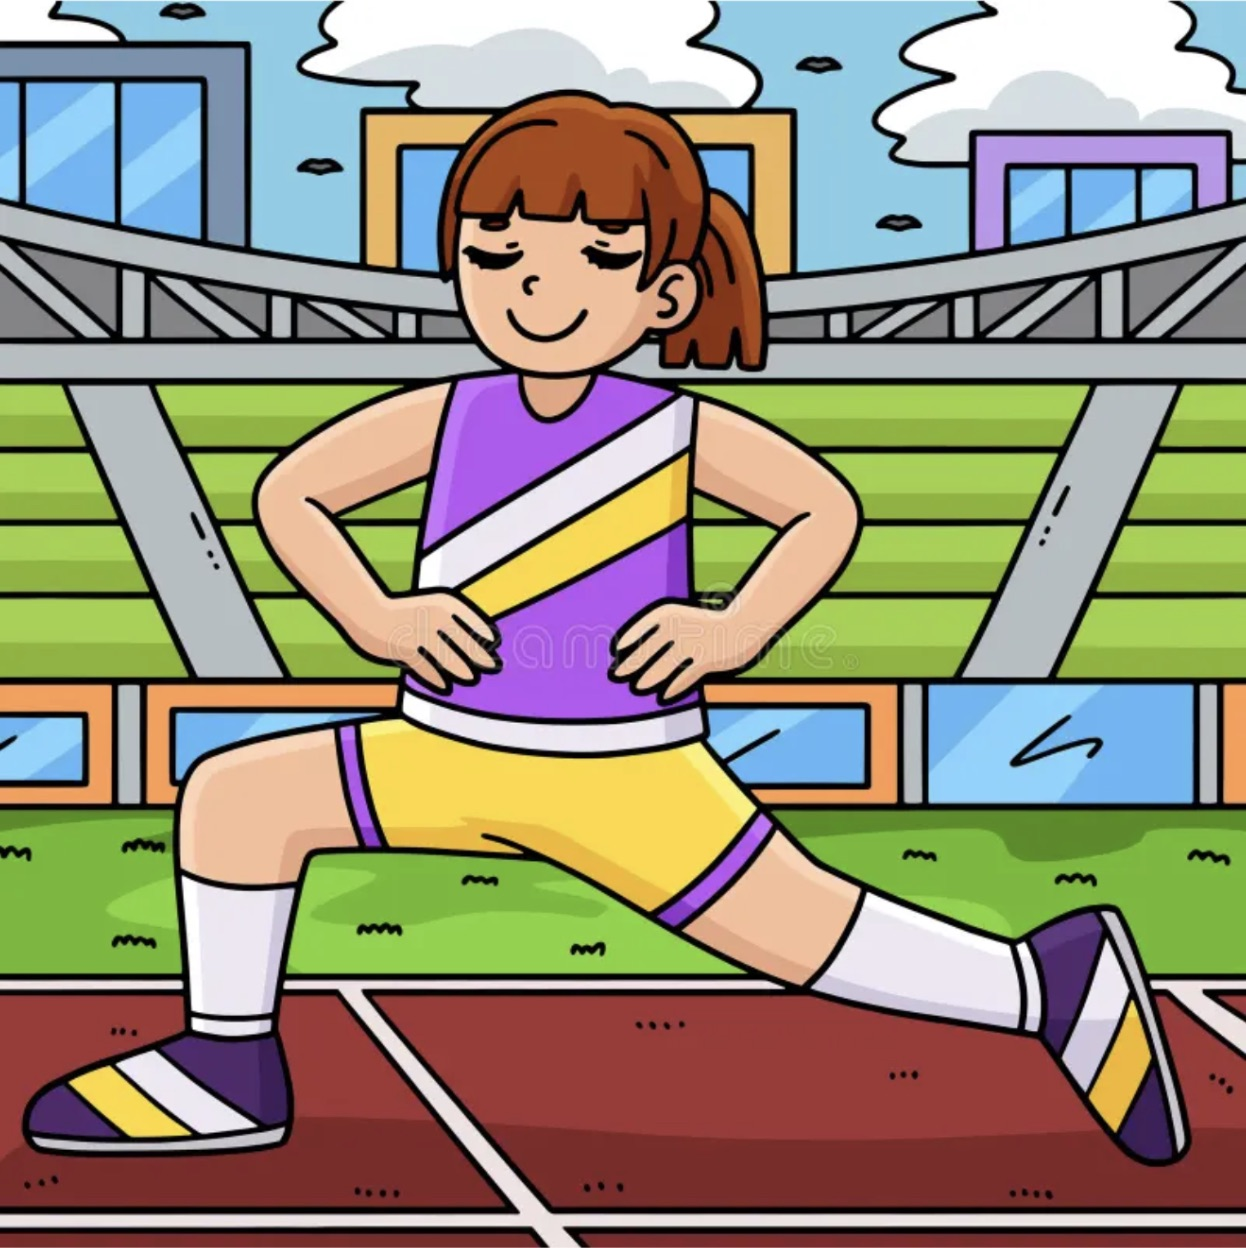
\includegraphics[width=0.25\textwidth]{girl.jpeg} & \textbf{Samantha, 25 yrs old} \\ 
    \hline
    \textbf{Context} &
    \begin{itemize}[leftmargin=*]
        \item Weekend yoga instructor and passionate barista
        \item Enjoys hiking, taking care of her plants, and spending time with friends
        \item Got into car accident and injured hand; lost a lot of strength and mobility because of prolonged cast duration
    \end{itemize} \\
    \hline
    \textbf{Goals} &
    \begin{itemize}[leftmargin=*]
        \item Remain consistent to regain hand mobility
    \end{itemize} \\
    \hline
    \textbf{What does this entail} &
    \begin{itemize}[leftmargin=*]
        \item Struggles with progressing and sticking to physical therapy routine due to active/busy schedule
        \item Stiff/weak joints, time sensitive to regain strength and mobility
        \item Will allow her to progress without losing progress
    \end{itemize} \\
    \hline
\end{longtable}


\begin{longtable}{|p{0.3\textwidth}|p{0.7\textwidth}|}
    \caption{User Persona: Tom} \label{table:user_persona_tom} \\
    \hline
    \multicolumn{2}{|c|}{\textbf{End User}} \\ 
    \hline
    \endfirsthead

    \hline
    \multicolumn{2}{|c|}{\textbf{End User} (continued)} \\ 
    \hline
    \endhead

    \hline
    \multicolumn{2}{|r|}{\textit{Continued on next page}} \\ 
    \hline
    \endfoot

    \hline
    \endlastfoot

    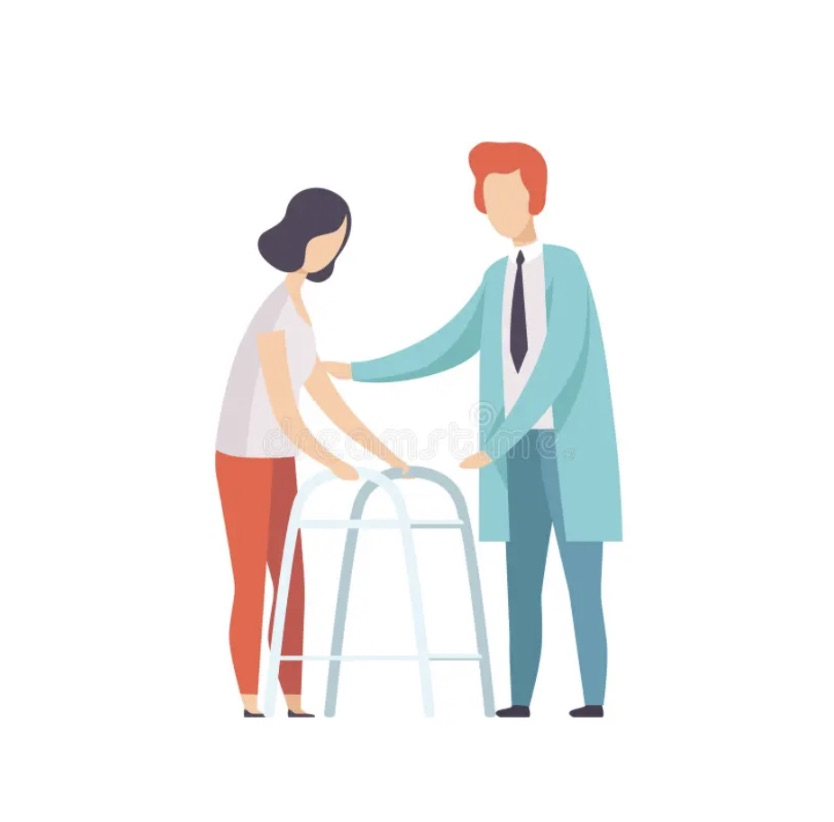
\includegraphics[width=0.25\textwidth]{tom.jpeg} & \textbf{Tom, 42 yrs old} \\ 
    \hline
    \textbf{Context} &
    \begin{itemize}[leftmargin=*]
        \item Physical therapist 
        \item Passionate about helping his clients the best he can
    \end{itemize} \\
    \hline
    \textbf{Goals} &
    \begin{itemize}[leftmargin=*]
        \item Be able to prescribe exercises and track progress remotely with potentially stubborn clients
        \item Retain clients who otherwise would cancel therapy altogether
    \end{itemize} \\
    \hline
    \textbf{What does this entail} &
    \begin{itemize}[leftmargin=*]
        \item Understands that clients have a hard time making it to appointments and not everyone can afford to see him often
    \end{itemize} \\
    \hline
\end{longtable}


\subsection{Clients}

\begin{longtable}{|p{0.3\textwidth}|p{0.7\textwidth}|}
    \caption{Client: Insurance Company} \label{table:client_insurance} \\
    \hline
    \multicolumn{2}{|c|}{\textbf{Client}} \\ 
    \hline
    \endfirsthead

    \hline
    \multicolumn{2}{|c|}{\textbf{Client} (continued)} \\ 
    \hline
    \endhead

    \hline
    \multicolumn{2}{|r|}{\textit{Continued on next page}} \\ 
    \hline
    \endfoot

    \hline
    \endlastfoot

    
\includegraphics[width=0.25\textwidth]{insurance.jpeg} & \textbf{Insurance Company} \\ 
    \hline
    \textbf{Context} &
    \begin{itemize}[leftmargin=*]
        \item Mid-size health insurance company 
        \item For-profit company
        \item Wants to buy product to provide a service at a cheaper price
        \item Increase retention rate for provided service
    \end{itemize} \\
    \hline
    \textbf{Goals} &
    \begin{itemize}[leftmargin=*]
        \item To provide affordable healthcare to the average person
        \item Allow more accessibility to physical therapy exercises
    \end{itemize} \\
    \hline
    \textbf{What does this entail} &
    \begin{itemize}[leftmargin=*]
        \item Replacing physical therapy visits
        \item Increasing more End Users to have access to in-person therapy meetings
    \end{itemize} \\
    \hline
\end{longtable}


\end{document}
